\documentclass[11pt a4paper]{article}
\usepackage[margin=2cm]{geometry}
\usepackage{amsmath, amssymb}
\usepackage{graphicx}
\usepackage{float}
\usepackage{aligned-overset}

% partielle ableitungen
\newcommand{\delr}{\partial_r}
\newcommand{\deltheta}{\partial_\theta}
\newcommand{\delphi}{\partial_\varphi}

% elektrische feldkonstante
\newcommand{\epsz}{\epsilon_0}
% 1 / 4pi eps
\newcommand{\kco}{\frac{1}{4\pi\epsilon_0}}

% fancy header
\usepackage{fancyhdr}
\fancyhf{}
% vspaces in den headern fuer Distanzen notwendig
% linke Seite: Namen der Abgabegruppe
\lhead{\textbf{Matthias Maile\\Roman Surma}\vspace{1.5cm}}
% rechte Seite: Modul, Gruppe, Semester
\rhead{\textbf{Physik II - Gruppe 2\\Sommersemester 2020}\vspace{1.5cm}}
% Center: nr. des blattes
\chead{\vspace{2.5cm}\huge{\textbf{16. Übungsblatt}}}
% benoetigt damit der eigentliche Text nicht in der Überschrift steckt
\setlength{\headheight}{4cm}

% zum zeichnen tikz
\usepackage{tikz}

\begin{document}
\thispagestyle{fancy}
\section*{Aufgabe 1: Eine geladene Linie}
\par{a)}
Die dreidimensionale Linienladungsdichte $\rho$ lautet:
\[
	\rho(\vec r) =
	\sigma \cdot \delta(x) \cdot \delta(y) \cdot 
	\Theta\left( z + \frac a 2 \right)
	\cdot \Theta\left(\frac a 2 - z\right)
	\qquad \text{ mit } \sigma \text{ als Linienladungsdichte }
	\sigma = \frac Q a
\]

\par{b)}
Aus der Multipolentwicklung folgt:
\begin{align*}
	\phi (\vec r) 
	&= \kco 
	\int_{\mathbb{R}^3} \frac{\rho(\vec r^\prime)}
	{\vert \vec r - \vec r^\prime \vert} 
	d^3r^\prime \\
	% rho einsetzen
	&= \kco
	\int_{-\infty}^\infty
	\int_{-\infty}^\infty
	\int_{-\infty}^\infty
	\frac{
	\sigma \cdot \delta(x^\prime) \cdot \delta(y^\prime) \cdot 
	\Theta\left( z^\prime + \frac a 2 \right)
	\cdot \Theta\left(\frac a 2 - z^\prime \right)}
	{\sqrt{(x-x^\prime)^2 + (y-y^\prime)^2 + (z-z^\prime)^2}} \
	dx^\prime dy^\prime dz^\prime\\
	% x und y integrieren
	&= \frac{Q}{4\pi\epsz a} \int_{-\frac a 2}^{\frac a 2}
	\frac1{\sqrt{x^2 + y^2 + (z-z^\prime)^2}} \ dz^\prime \\
	% r und u einbringen
	^{r^2 := x^2 + y^2}
	_{u := z - z^\prime}
	\Rightarrow
	&= \frac{-Q}{4\pi\epsz a} \int_{z+\frac a 2}^{z-\frac a 2}
	\frac1{\sqrt{r^2 + u^2}} \ du \\
	% umformen fuer zweite substitution
	&= \frac{-Q}{4\pi\epsz a} \int_{z+\frac a 2}^{z-\frac a 2}
	\frac{1}{u + \sqrt{r^2 + u^2}}
	\frac{u + \sqrt{r^2 + u^2}}{\sqrt{r^2 + u^2}} 
	\ du \\
	% weiter umformen
	&= \frac{-Q}{4\pi\epsz a} \int_{z+\frac a 2}^{z-\frac a 2}
	\frac{1}{u + \sqrt{r^2 + u^2}}
	\left( 1 + \frac{u}{\sqrt{r^2 + u^2}} \right)
	\ du \\
	% 2. substitution
	v:= u+\sqrt{r^2 + u^2} \quad
	du = \frac{dv}{1 + \frac{u}{\sqrt{r^2 + u^2}}}
	\Rightarrow
	&= \frac{-Q}{4\pi\epsz a} \int_{v_1}^{v_2}
	\frac{1}{v}
	\ dv \\
	% integrieren
	&= \frac{-Q}{4\pi\epsz a}
	\ln \left( \frac{v_2}{v_1} \right) \\
	% negatives vorzeichen wegstreichen
	&= \frac{Q}{4\pi\epsz a}
	\ln \left( \frac{v_1}{v_2} \right) \\
	% ruecksubstituieren
	&= \frac{Q}{4\pi\epsz a}
	\ln \left( \frac{
		z+\frac a 2 + \sqrt{x^2 + y^2 + \left(z+\frac a 2\right)^2}}
	{
		z-\frac a 2 + \sqrt{x^2 + y^2 + \left(z-\frac a 2\right)^2}}
	\right)
\end{align*}

\newpage
\setlength{\headheight}{0cm}
c)
\begin{enumerate}
	\item $x = y = 0$, $z \rightarrow \frac a 2$
		\[
			\phi(z \rightarrow \frac a2) =
			\lim_{z\rightarrow\frac a2} \frac{Q}
			{4\pi\epsz a} \ln\left(\frac{
				z + \frac a2 + \sqrt{\left(z+\frac a2
				\right)^2}}{
				z - \frac a2 + \sqrt{\left(z-\frac a2
				\right)^2}}
			\right)
		=
			\lim_{z\rightarrow\frac a2} \frac{Q}
			{4\pi\epsz a} \ln\left(\frac{2z + a}{2z -a }
			\right)
		\]
	% x achse, nahe bei null
	\item $\vec r \in x\text{-Achse}$
	\[
		\phi(x) = \frac{Q}{4\pi\epsz a} \ln\left(\frac{
			\frac a2 + \sqrt{x^2 + \frac{a^2}4}}{
			-\frac a2 + \sqrt{x^2 + \frac{a^2}4}}\right)
		=
		\frac{Q}{4\pi \epsz a} \ln\left(\frac{
			x^2}{\left(\sqrt{x^2 + \frac{a^2}{4}} - 
			\frac{a^2}{4}\right)^2} \right)
			\]
	\item $r_z = 0$, $r \gg \frac a2$
		\[
			\phi(r) = \frac{Q}{4\pi\epsz a} \ln\left(\frac{
				\frac a2 + \sqrt{r^2 + \frac{a^2}{4}}}{
				-\frac a2 + \sqrt{r^2 + \frac{a^2}{4}}}
			\right)
			\overset{r \gg \frac a2}{\approx}
			\frac{Q}{4\pi\epsz a} \ln\left(\frac{
				r + \frac a 2}{r - \frac a2}\right)
		\]
\end{enumerate}

\newpage
\setlength{\headheight}{0cm}

\section*{Aufgabe 2: Ladungsverteilung und Multipolmomente}
\quad \par{a)}
\[
	\rho (\vec r) = q \cdot \delta(x) \delta(y) \cdot \left(
	\delta(z+a) + \delta(z-a) - 2\delta(z) \right)
\]
\par{b)}
\begin{align*}
	\phi(\vec r) = \frac1{4\pi\epsz} \int_{\mathbb{R}^3} 
	\frac{\rho(r)}{\vert \vec r - \vec r^\prime \vert} d^3r^\prime
	% rho einsetzen
	&= \frac{1}{4\pi\epsz} 
	\int_{-\infty}^\infty
	\int_{-\infty}^\infty
	\int_{-\infty}^\infty
	\frac{
	q \cdot \delta(x^\prime) \delta(y^\prime) \cdot \left(
	\delta(z^\prime+a) + \delta(z^\prime-a) - 2\delta(z^\prime) \right)}
	{\sqrt{(x-x^\prime)^2 +(y-y^\prime)^2 + (z-z^\prime)^2}}
	\ dx^\prime dy^\prime dz^\prime \\
	%  x und y integrieren (durch delta distribution)
	&= \frac{q}{4\pi\epsz} 
	\int_{-\infty}^\infty 
	\frac{\delta(z^\prime+a) + \delta(z^\prime-a) - 2\delta(z^\prime)}
	{\sqrt{x^2 + y^2 + (z - z^\prime)^2}}
	\ dz^\prime \\
	% z integrieren und integral aufteilen
	&= \frac{q}{4\pi\epsz} \left[
		\frac{1}{\sqrt{x^2 + y^2 + (z-a)^2}} + 
		\frac{1}{\sqrt{x^2 + y^2 + (z+a)^2}} -
		\frac{2}{\sqrt{x^2 + y^2 + z^2}}  
	\right] \\
	% r^2 = x^2 + y^2 einbringen
	r := \sqrt{x^2 + y^2}
	\Rightarrow
	&= \frac{q}{4\pi\epsz} \left[
		\frac{1}{\sqrt{r^2 + (z-a)^2}} + 
		\frac{1}{\sqrt{r^2 + (z+a)^2}} -
		\frac{2}{\sqrt{r^2 + z^2}}  
	\right] \\
	% r ausklammern
	&= \frac{q}{4\pi\epsz} \frac1r \left[
		\frac{1}{\sqrt{1 + \left( \frac{z-a}{r} \right)^2}} +
		\frac{1}{\sqrt{1 + \left( \frac{z+a}{r} \right)^2}} -
		\frac{2}{\sqrt{1 + \left( \frac{z}{r} \right)^2}} 
	\right] \\
	% taylor
	\text{Taylor} \Rightarrow
	&= \frac{q}{4\pi\epsz} \frac1r * [
			% erster bruch als taylor reihe
			1 + \frac{1}{2} \left(\frac{z-a}{r}\right)^2
			+ \frac{3}{8} \left(\frac{z-a}{r}\right)^4
			+  \dotsb \\
			% zweiter bruch
			&\hspace{1.49cm} +
			1 + \frac{1}{2} \left(\frac{z+a}{r}\right)^2
			+ \frac{3}{8} \left(\frac{z+a}{r}\right)^4
			+  \dotsb \\
			% 3. bruch
			&\hspace{1.49cm} -
			2 - \frac{2}{2} \left(\frac{z}{r}\right)^2
			\hspace{0.7cm}
			-\frac{6}{8} \left(\frac{z}{r}\right)^4
			\hspace{0.7cm} +  \dotsb] \\
	% zusammen fassen
	&= \frac{q}{4\pi\epsz} \left[
		\underbrace{\frac{1+1-2}{r}}_{0} +
		\underbrace{\frac{(z-a)^2 + (z+a)^2 - 2z^2}{2 r^3}}_{
			\frac{a^2}{r^3}}
		+ 
		\underbrace{\frac{3 (z-a)^4 + 3 (z+a)^4 - 6 z^4}{8 r^5}}_{
			\frac{9a^2 z^2 + a^4}{4r^5}} + \dotsb
		\right] \\
	% weiter zusammen fassen
	&= \frac{q a^2}{4\pi\epsz} \left(
	\frac{1}{r^3} + \frac{z^2 + a^2}{4r^5} \right)
\end{align*}

Das erste nicht-verschwindene Moment ist damit das Quadrupolmoment
\[
	Q(\vec e_r) = qa^2
\]

c)
Aus dem Quadrupolmoment folgt das Potential:
\[
	\phi (r) = \frac{Q(\vec e_r)}{4\pi\epsz r^3} 
	= \frac{qa^2}{4\pi\epsz r^3}
\]


	


\newpage
\section*{Aufgabe 3: Spiegelladungen}

a)
Zum Erfüllen der Randbedingung setzen 3 weitere Ladungen in das System,
die gegenüberliegende Ladung ist gleichnamig. Die Ladungen im 2. und im 4.
Quadranten sind jedoch negativ geladen. Die Anordnung sieht dann wie folgt
aus:
\newline
\begin{center}
\begin{tikzpicture}
	% die x und y achse
	\draw[gray, thick, ->] (0, -3) -- (0, 3);
	\draw[gray, thick, ->] (-5, 0) -- (5,0);
	% die Ladungen mit annotation
	\filldraw [black] (3,2) circle (2pt);
	\draw (3,2) node [right] {$Q$};
	\filldraw [black] (-3,2) circle (2pt);
	\draw (-3,2) node [left] {$-q$};
	\filldraw [black] (-3,-2) circle (2pt);
	\draw (-3,-2) node [left] {$q$};
	\filldraw [black] (3,-2) circle (2pt);
	\draw (3,-2) node [right] {$-q$};
	% weg zu Ladung q0
	\draw[thick, dashed] (3,0) -- (3,2);
	\draw[thick, dashed] (0,2) -- (3,2);
	% anotation an der achse
	\draw (0,2) node [left] {$b$};
	\draw (3,0) node [below] {$a$};
\end{tikzpicture}
\end{center}
Durch die Multipolentwicklung können wir das elektrische Potential im Raum ermitteln:
\begin{align*}
	\phi (\vec r)
	&= \frac1{4\pi\epsz} \sum_i \frac{q_i}{d(\vec r, \vec{q_i})} \\
	% ladungen und distanzen einsetzen
	&= \kco \left[
		\underbrace{\frac{Q}{\sqrt{(x-a)^2 + (y-b)^2}}}_{
			\text{Durch Ladung } Q}
		- \underbrace{\frac{Q}{\sqrt{(x+a)^2 + (y-b)^2}} }_{
			\text{Spiegelladung im 2. Quadrant}}
		+ \underbrace{\frac{Q}{\sqrt{(x + a)^2 + (y+b)^2}} }_{
			\text{Spiegelladung im 3. Quadrant}}
		- \underbrace{\frac{Q}{\sqrt{(x-a)^2 + (y+b)^2}} }_{
			\text{Spiegelladung im 4. Quadrant}}
	\right]
\end{align*}
Die Randbedingung $\phi = 0$ auf den Platten ist damit auch erfüllt:
\begin{align*}
	\phi \left( \begin{pmatrix} x \\ 0 \end{pmatrix} \right) 
	&= \kco \left[
		\frac{Q}{\sqrt{(x-a)^2 + (0-b)^2}}
		- \frac{Q}{\sqrt{(x+a)^2 + (0-b)^2}}
		+ \frac{Q}{\sqrt{(x + a)^2 + (0+b)^2}}
		- \frac{Q}{\sqrt{(x-a)^2 + (0+b)^2}}
	\right] \\
	% zusammen fassen, 0 entfernen
	&= \kco \left[
		\frac{Q}{\sqrt{(x-a)^2 + b^2}}
		- \frac{Q}{\sqrt{(x+a)^2 + b^2}}
		+ \frac{Q}{\sqrt{(x + a)^2 + b^2}}
		- \frac{Q}{\sqrt{(x-a)^2 + b^2}}
	\right] \\
	&= 0 \\
	% jetzt noch mal alles für y achse
	\phi \left( \begin{pmatrix} 0 \\ y \end{pmatrix} \right) 
	&= \kco \left[
		\frac{Q}{\sqrt{(0-a)^2 + (y-b)^2}}
		- \frac{Q}{\sqrt{(0+a)^2 + (y-b)^2}}
		+ \frac{Q}{\sqrt{(0 + a)^2 + (y+b)^2}}
		- \frac{Q}{\sqrt{(0-a)^2 + (y+b)^2}}
	\right] \\
	% 0 entfernen
	&= \kco \left[
		\frac{Q}{\sqrt{a^2 + (y-b)^2}}
		- \frac{Q}{\sqrt{a^2 + (y-b)^2}}
		+ \frac{Q}{\sqrt{a^2 + (y+b)^2}}
		- \frac{Q}{\sqrt{a^2 + (y+b)^2}}
	\right] \\
	&= 0
\end{align*}

\newpage
b) 
Für den Bewewis der Eindeutigkeit nehmen wir an, dass zwei Lösungen,
$\phi_1$ und $\phi_2$ existieren. Die Differenz der Potentiale definieren 
wir als $\phi_0 = \phi_1 - \phi_2$.\\
Aus dem ersten Greenschen Satz folgt dann:
\begin{align*}
	\int_V (\vec \nabla \phi_0)^2 \ d^3r
	+ \underbrace{
		\int_V \phi_0 \cdot \Delta \phi_0 \ d^3 r}_{
		^\text{$\Delta \phi_0 = \Delta \phi_1 - \Delta \phi_2$}
		_\text{$= -\frac{\rho}{\epsz} + \frac{\rho}{\epsz} = 0$}}
	&= 
	\underbrace{\int_{\partial V} \phi_0 \cdot \partial_n \phi_0 \ d^2r}
	_{^{=0 \text{, wegen Dirichlet Rdb muss}}
	_{\text{ $\phi_0(\vec r) \vert_{r\in \partial V} =0$ gelten}}}
	\\
	% folgerung
	\int_V (\vec \nabla \phi_0)^2 \ d^3r 
	+ \hspace{1.1cm} 0 \hspace{1.1cm} &= \hspace{1.2cm} 0
\end{align*}
In der 2. Zeile wird das $\vec E$-Feld des Differenzfeldes $\phi_0$ 
quadriert und, muss also $\geq0$ sein. \\
Da über eine nicht negative Zahl integriert wird, muss der Wert des
Integrals auch positiv sein. Aufgrund der Poisson-Gleichung und der 
Dirichlet-Randbedingung ist dieser aber 0, d.h. dass auch das $\vec E$-Feld 
im gesamten Raum 0 ist. \\
\[
	\int_V (\vec \nabla \phi_0)^2 \ d^3r = 0
	\Rightarrow
	\int_V (\vec E(\vec r))^2 \ d^3r = 0
	\Rightarrow
	\vec E (\vec r) = 0, \text{ für } \vec r \in V
\]
Dies stellt keine sinnvolle Lösung für die Poissongleichung dar, weshalb 
keine zwei Lösungen existieren können.

\newpage

\begin{figure}[H]
	\centering
	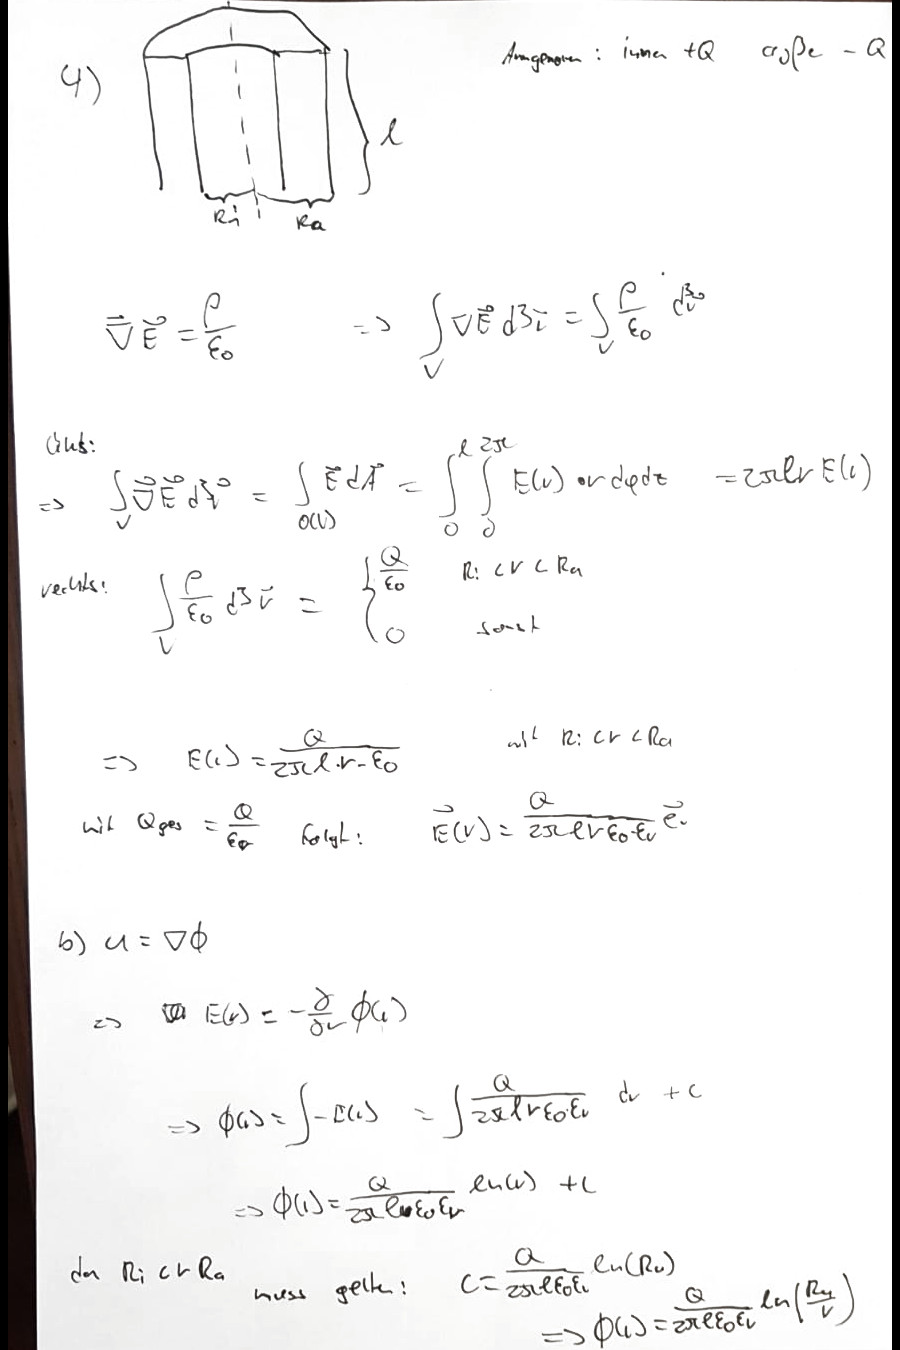
\includegraphics[width=15cm]{aufgabe4_1_cleaned.jpg}
\end{figure}
\newpage

\begin{figure}[H]
	\centering
	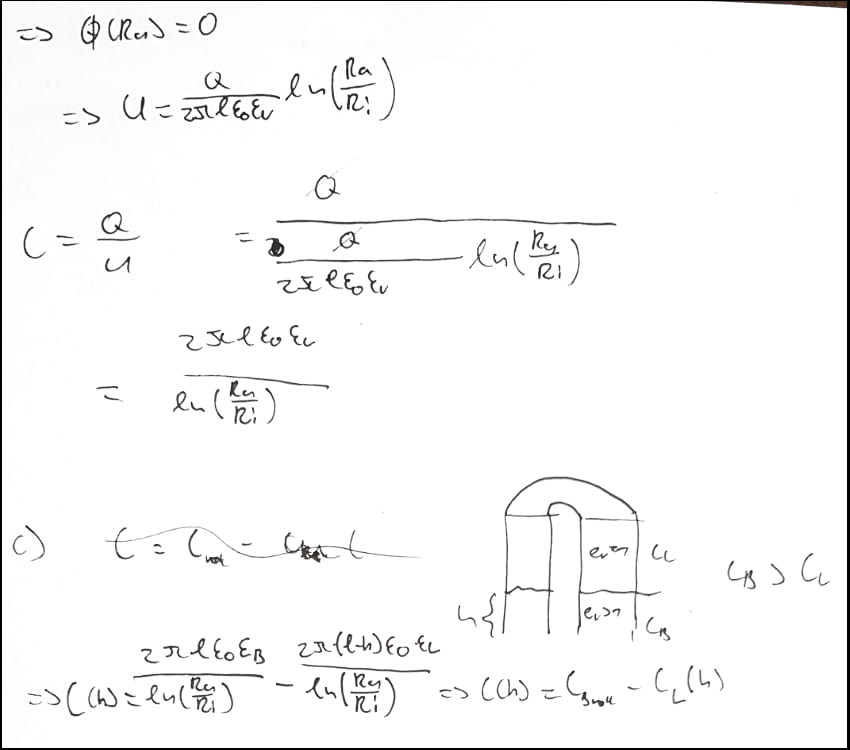
\includegraphics[width=15cm]{aufgabe4_2_cleaned.jpg}
\end{figure}
\newpage

\section*{Aufgabe 5: Greensche Funktion}
Sei $D$ ein $n$-dimensionaler Differentialoperator und $G$ eine Greensche Funktion, sodass 
gilt:
\[
	DG(\vec x) = \delta^{(n)}(\vec x), \hspace{1cm} x \in \mathbb{R}^n
\]
a) Eine partikuläre Lösung $f_p(\vec x)$ der Differentialgleichung
\[
	Df(\vec x) = J(\vec x)
\]

mit Inhomogenität $J(\vec x)$ kann durch Faltung der Inhomogenität mit der
Greenschen Funktion erzeugt werden:
\begin{align*}
	D f_p(\vec x) 
	&= J(\vec x) \\
	% mit delta funktion ins integral verwandeln
	&= \int_{\mathbb{R}^n} J(\vec x^\prime)
	\delta(\vec x - \vec x^\prime) d^nx^\prime \\
	% delta umstellen zu DG(x)
	&= \int_{\mathbb{R}^n} J(\vec x^\prime) 
	DG(\vec x - \vec x^\prime) d^nx^\prime \\
	% D rausziehen
	&= D \int_{\mathbb{R}^n} J(\vec x^\prime)
	G(\vec x - \vec x^\prime) d^nx^\prime \\
	% D entfernen
	\Rightarrow
	f_p(\vec x) 
	&=  \int_{\mathbb{R}^n} J(\vec x^\prime)
	G(\vec x - \vec x^\prime) d^nx^\prime
\end{align*}
Der Sprung zwischen der 3. und 4. Zeile folgt daraus, dass $D$ nach $\vec x$
ableitet, weshalb $J(\vec x^\prime)$ wie ein linearfaktor behandelt werden
kann. \newline
\vspace{0.5cm}
b) Die Heaviside (Theta-Funktion)
\[
	\Theta (x) = \begin{cases} 
		1 &\text{für } x \geq 0\\
		0 &\text{für } x < 0
	\end{cases}
\]
c) 1.
\[
	\rho (r) = Q \cdot \delta^3(\vec r) 
	= Q \cdot \delta(x) \cdot \delta(y) \cdot \delta(z)
\]

2.
\begin{align*}
	\int \vec E \ d\vec A = \frac{Q_\text{enq}}{\epsz}
	&= \frac{Q}{\epsz} \int \delta^3(\vec r^\prime) d^3 \vec r^\prime \\
	% umformen
	E \cdot 4\pi r^2 &= \frac{Q}{\epsz} \\
	% nach E umstllen
	E &= \frac{Q}{4\pi r^2 \epsz}
\end{align*}

Da wir uns in einem Radialfeld befinden:
\begin{align*}
	-\nabla \phi = -\partial_r \phi
	&= E(r) \\
	% integral
	\Leftrightarrow
	\phi &= - \int_\infty^r \frac{Q}{4\pi r^{\prime 2} \epsz} dr^\prime
	\\
	&= \frac{Q}{4\pi\epsz} \frac1r
\end{align*}

3.
\begin{align*}
	\phi(r) 
	&= \int_{\mathbb{R}^3} \frac{-\rho(\vec r^\prime)}{\epsz} 
	\cdot G(\vec r - \vec r^\prime) \ d^3r^\prime \\
	% rho einsetzen
	\frac{Q}{4\pi \epsz r}
	&= \int_{\mathbb{R}^3} Q \cdot \delta^3(\vec r^\prime)
	\cdot G(\vec r - \vec r^\prime) \ d^3r^\prime \\
	% integrieren
	G(r) &= \frac1{4\pi \epsz r}
\end{align*}

4.
\begin{align*}
	\phi (\vec r) 
	&= \int_{\mathbb{R}^3} \rho(\vec r^\prime) G(\vec r - \vec r^\prime)
	d^3r^\prime \\
	% G einsetzen
	\overset{(3.)}&{=} \int_{\mathbb{R}^3} \rho(\vec r^\prime) \cdot
	\frac1{4\pi\epsz} \cdot \frac1 {\vert \vec r - 
	\vec r^\prime \vert}
	d^3r^\prime \\
	% 1/4pieps rausziehen
	&= \kco \int_{\mathbb{R}^3}
	\frac{\rho(\vec r^\prime)} {\vert \vec r - 
	\vec r^\prime \vert}
	d^3r^\prime \\
\end{align*}

\end{document}
